\documentclass[11pt,a4paper]{article}

\usepackage[utf8]{inputenc}
\usepackage[T1]{fontenc}
\usepackage{lmodern}
\usepackage[top=1.8cm, bottom=1.8cm, left=2cm, right=2cm]{geometry}
\usepackage{graphicx}
\usepackage[export]{adjustbox}
\usepackage{booktabs}
\usepackage{xcolor}
\usepackage{listings}
\usepackage{hyperref}
\usepackage{microtype}
\usepackage{titlesec}

% Colors
\definecolor{primaryblue}{RGB}{20, 60, 110}
\definecolor{codegray}{RGB}{247, 248, 250}
\definecolor{bordergray}{RGB}{200, 205, 215}

% Compact section formatting
\titleformat{\section}{\large\bfseries\color{primaryblue}}{}{0pt}{}[\vspace{-2pt}\titlerule]
\titlespacing*{\section}{0pt}{10pt}{4pt}
\titleformat{\subsection}{\normalsize\bfseries\color{primaryblue}}{}{0pt}{}
\titlespacing*{\subsection}{0pt}{6pt}{2pt}

% Code Listing Configuration
\lstset{
    backgroundcolor=\color{codegray},
    basicstyle=\ttfamily\scriptsize,
    breaklines=true,
    breakatwhitespace=true,
    frame=single,
    rulecolor=\color{bordergray},
    keywordstyle=\bfseries\color{primaryblue},
    tabsize=2,
    showstringspaces=false,
    aboveskip=4pt,
    belowskip=4pt
}

\setlength{\parindent}{0pt}
\setlength{\parskip}{3pt}

\begin{document}

% ------------------------------------------------------------------------------
% HEADER (Simple Homework / Compte Rendu Header)
% ------------------------------------------------------------------------------
\begin{center}
    {\LARGE \textbf{Technical Execution Report: Apache Hive \& Hadoop}}\\[4pt]
    {\large \textbf{Workload 1: Los Angeles Crime Data Analysis (1M+ Records)}}\\[6pt]
    \normalsize
    \textbf{Platform:} Apache Hadoop 3.3.6 \quad \vline \quad \textbf{Engine:} Apache Hive 4.0.1 (MapReduce/MR3)\\[2pt]
    \textit{Distributed Infrastructure \& Analytical Data Architectures}
\end{center}
\vspace{-4pt}
\hrule height 1.2pt
\vspace{8pt}

% ------------------------------------------------------------------------------
\section*{1. Chargement des Données dans HDFS}
% ------------------------------------------------------------------------------
\textbf{Objectif :} Ingestion du fichier brut \texttt{Crime\_Data\_from\_2020\_to\_2024.csv} (243.6 Mo, 1,004,894 lignes) dans l'environnement distribué HDFS sous le répertoire de staging \texttt{/data/crime/raw}.

\begin{lstlisting}[language=bash]
hdfs dfs -mkdir -p /data/crime/raw
hdfs dfs -put -f /vagrant/data/Crime_Data_from_2020_to_2024.csv /data/crime/raw/
hdfs dfs -ls -h /data/crime/raw/
\end{lstlisting}

\begin{center}
    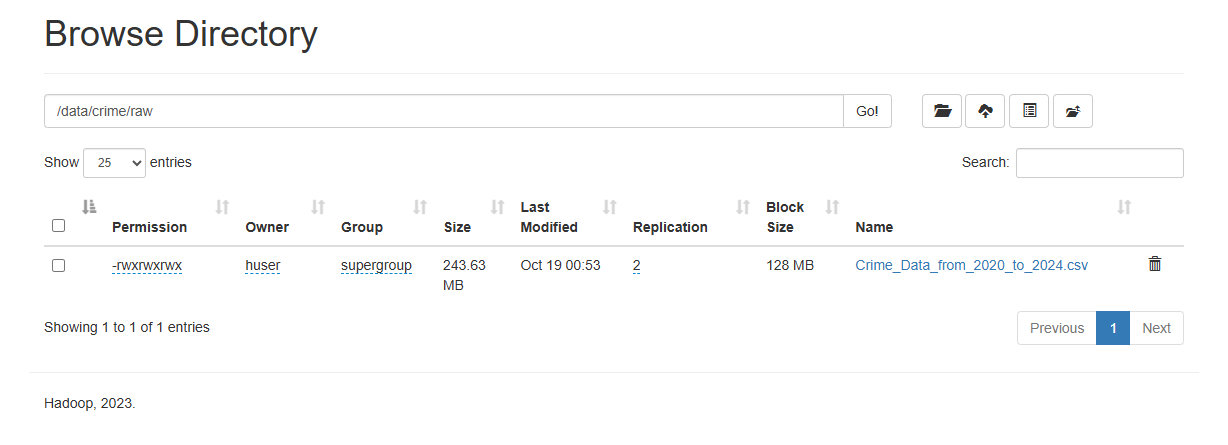
\includegraphics[max width=0.92\linewidth, max height=5.2cm, keepaspectratio]{images/ex1_01_hdfs_upload.png}
\end{center}
\textbf{Résultat :} Le fichier est bien stocké dans HDFS avec un facteur de réplication de 2 et une taille de 243.63 Mo.

% ------------------------------------------------------------------------------
\section*{2. Création de la Table Externe avec OpenCSVSerde}
% ------------------------------------------------------------------------------
\textbf{Objectif :} Création de la base de données \texttt{crime\_data\_db} et de la table externe \texttt{crime\_data\_raw}. L'utilisation du SerDe \texttt{OpenCSVSerde} est obligatoire pour gérer correctement les virgules imbriquées dans les champs textuels entre guillemets (descriptions de crimes, adresses).

\begin{lstlisting}[language=SQL]
CREATE DATABASE IF NOT EXISTS crime_data_db;
USE crime_data_db;

CREATE EXTERNAL TABLE IF NOT EXISTS crime_data_raw (
    dr_no STRING, date_rptd STRING, date_occ STRING, time_occ STRING,
    area STRING, area_name STRING, rpt_dist_no STRING, part_1_2 STRING,
    crm_cd STRING, crm_cd_desc STRING, mocodes STRING, vict_age STRING,
    vict_sex STRING, vict_descent STRING, premis_cd STRING, premis_desc STRING,
    weapon_used_cd STRING, weapon_desc STRING, status STRING, status_desc STRING,
    crm_cd_1 STRING, crm_cd_2 STRING, crm_cd_3 STRING, crm_cd_4 STRING,
    location STRING, cross_street STRING, lat STRING, lon STRING
)
ROW FORMAT SERDE 'org.apache.hadoop.hive.serde2.OpenCSVSerde'
WITH SERDEPROPERTIES ("separatorChar" = ",", "quoteChar" = "\"", "escapeChar" = "\\")
STORED AS TEXTFILE LOCATION '/data/crime/raw'
TBLPROPERTIES ("skip.header.line.count"="1");
\end{lstlisting}

\begin{center}
    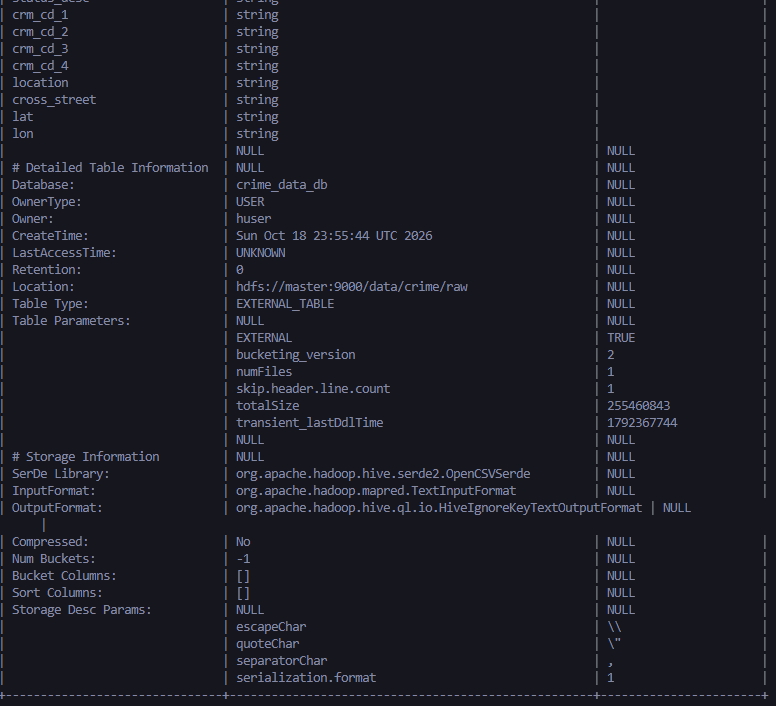
\includegraphics[max width=0.92\linewidth, max height=6.2cm, keepaspectratio]{images/ex1_02_create_table.png}
\end{center}
\textbf{Résultat :} La table est créée avec succès et la commande \texttt{DESCRIBE FORMATTED} confirme le paramétrage d'\texttt{OpenCSVSerde}.

% ------------------------------------------------------------------------------
\section*{3. Vérification des Échantillons (Sample Records)}
% ------------------------------------------------------------------------------
\textbf{Objectif :} Valider l'intégrité de la désérialisation en affichant les 5 premières lignes afin de confirmer l'absence de décalage de colonnes.

\begin{lstlisting}[language=SQL]
SELECT dr_no, date_occ, time_occ, area_name, crm_cd_desc, vict_age, vict_sex, status_desc 
FROM crime_data_raw LIMIT 5;
\end{lstlisting}

\begin{center}
    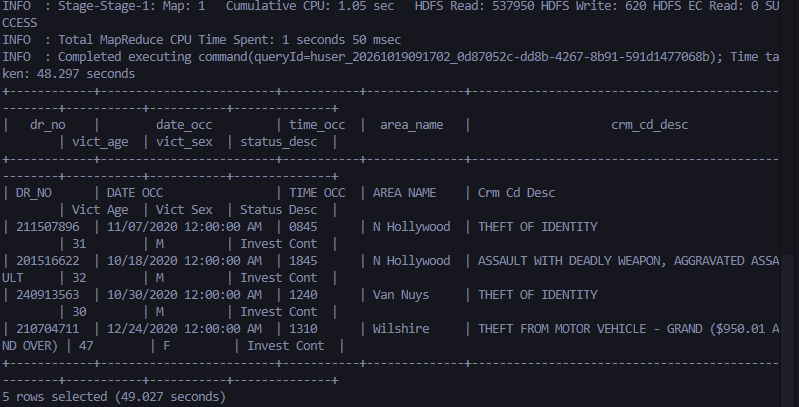
\includegraphics[max width=0.92\linewidth, max height=5.5cm, keepaspectratio]{images/ex1_03_sample_records.png}
\end{center}
\textbf{Résultat :} Les colonnes correspondent parfaitement aux données attendues sans décalage.

% ------------------------------------------------------------------------------
\section*{4. Nombre Total de Crimes et Unicité des Données}
% ------------------------------------------------------------------------------
\textbf{Objectif :} Vérifier le nombre total de lignes chargées ainsi que l'unicité de la clé primaire (\texttt{dr\_no}).

\begin{lstlisting}[language=SQL]
SELECT count(*) AS total_crimes, count(DISTINCT dr_no) AS unique_dr_no 
FROM crime_data_raw;
\end{lstlisting}

\begin{center}
    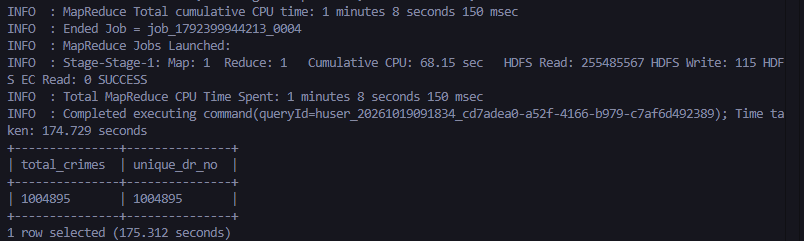
\includegraphics[max width=0.92\linewidth, max height=5.5cm, keepaspectratio]{images/ex1_04_total_crimes.png}
\end{center}
\textbf{Résultat :} Le dataset contient exactement \textbf{1,004,894} enregistrements (hors entête). Le nombre d'identifiants uniques est strictement égal à 1,004,894 (100\% d'unicité, aucun doublon).

% ------------------------------------------------------------------------------
\section*{5. Distribution Spatiale : Crimes par Zone Géographique}
% ------------------------------------------------------------------------------
\textbf{Objectif :} Identifier les zones de Los Angeles les plus touchées par les actes criminels (Top 10 des divisions LAPD).

\begin{lstlisting}[language=SQL]
SELECT area_name, count(*) AS crime_count 
FROM crime_data_raw 
GROUP BY area_name ORDER BY crime_count DESC LIMIT 10;
\end{lstlisting}

\begin{center}
    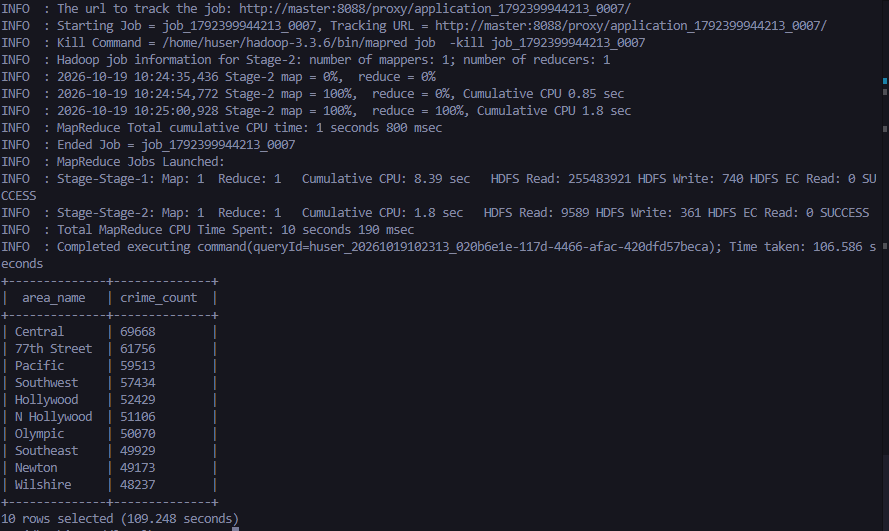
\includegraphics[max width=0.92\linewidth, max height=5.5cm, keepaspectratio]{images/ex1_05_crimes_by_area.png}
\end{center}
\textbf{Résultat :} La zone \textbf{Central} arrive en tête avec 69,668 crimes, suivie de \textbf{77th Street} (61,756) et \textbf{Pacific} (59,513).

% ------------------------------------------------------------------------------
\section*{6. Typologie Criminelle : Crimes les Plus Fréquents}
% ------------------------------------------------------------------------------
\textbf{Objectif :} Analyser les types d'infractions les plus récurrents dans la métropole.

\begin{lstlisting}[language=SQL]
SELECT crm_cd_desc, count(*) AS crime_count 
FROM crime_data_raw 
GROUP BY crm_cd_desc ORDER BY crime_count DESC LIMIT 10;
\end{lstlisting}

\begin{center}
    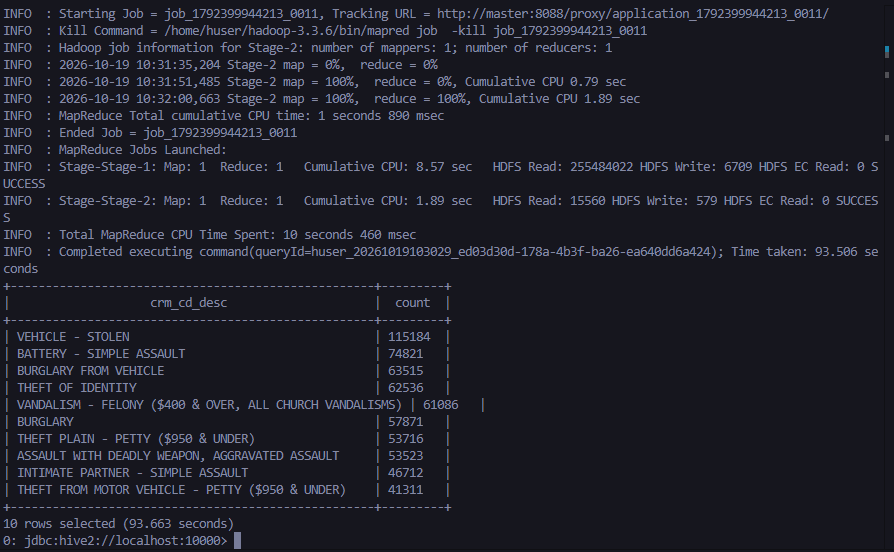
\includegraphics[max width=0.92\linewidth, max height=5.5cm, keepaspectratio]{images/ex1_06_common_crimes.png}
\end{center}
\textbf{Résultat :} Le vol de véhicule (\textbf{VEHICLE - STOLEN}) est l'infraction la plus courante avec 115,184 cas (plus de 11.4\% du total), suivi des agressions simples (\textbf{BATTERY - SIMPLE ASSAULT} : 74,821 cas).

% ------------------------------------------------------------------------------
\section*{7. Analyse Temporelle : Évolution Annuelle (2020--2024)}
% ------------------------------------------------------------------------------
\textbf{Objectif :} Étudier la dynamique des crimes par année sur la période 2020 à 2024.

\begin{lstlisting}[language=SQL]
SELECT substr(date_occ, 7, 4) AS crime_year, count(*) AS total_crimes 
FROM crime_data_raw 
WHERE substr(date_occ, 7, 4) IS NOT NULL AND length(substr(date_occ, 7, 4)) = 4 
GROUP BY substr(date_occ, 7, 4) ORDER BY crime_year ASC;
\end{lstlisting}

\begin{center}
    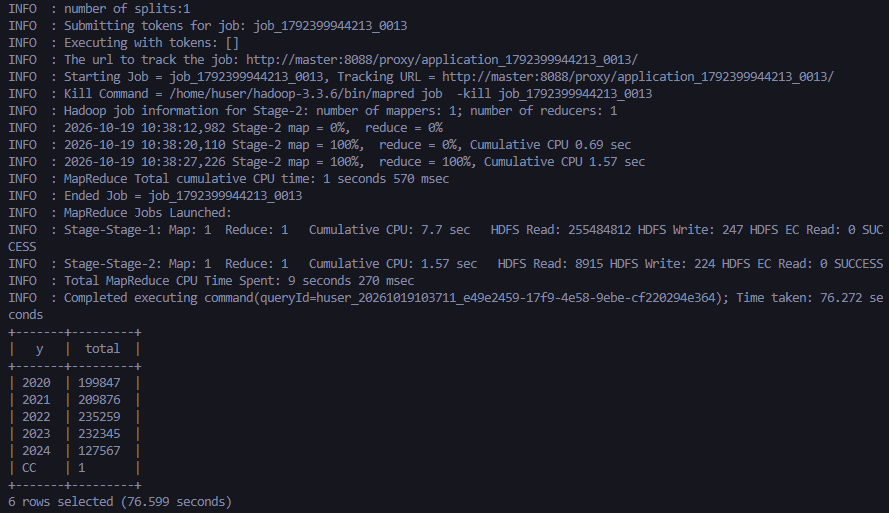
\includegraphics[max width=0.92\linewidth, max height=5.5cm, keepaspectratio]{images/ex1_07_crime_trends_year.png}
\end{center}
\textbf{Résultat :} Le volume a augmenté de 199,847 (2020) à un pic de \textbf{235,259} en 2022, avant de se stabiliser en 2023 (232,345). L'année 2024 (127,567) représente un jeu de données partiel jusqu'à mi-2024.

% ------------------------------------------------------------------------------
\section*{8. Filtrage par Arme : Crimes Impliquant une Arme de Poing}
% ------------------------------------------------------------------------------
\textbf{Objectif :} Isoler le nombre d'infractions commises à l'aide d'une arme de poing (\texttt{HAND GUN}).

\begin{lstlisting}[language=SQL]
SELECT count(*) AS total_handgun_crimes 
FROM crime_data_raw 
WHERE upper(trim(weapon_desc)) = 'HAND GUN';
\end{lstlisting}

\begin{center}
    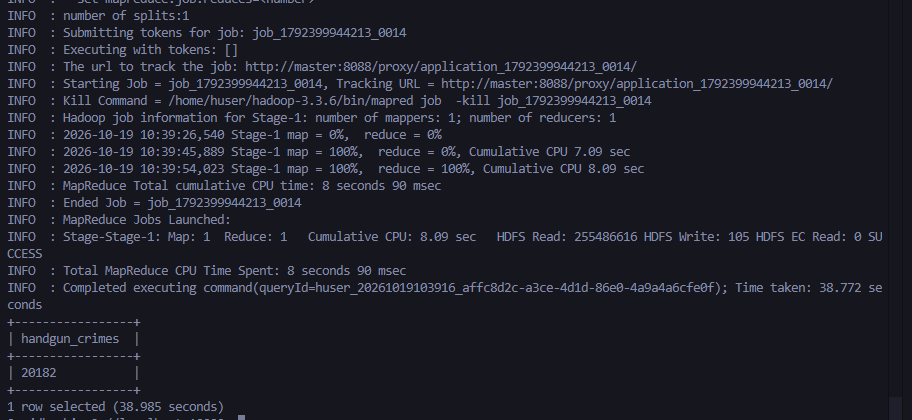
\includegraphics[max width=0.92\linewidth, max height=5.2cm, keepaspectratio]{images/ex1_08_handgun_filter.png}
\end{center}
\textbf{Résultat :} Exactement \textbf{20,182} crimes ont été perpétrés avec une arme de poing (HAND GUN).

% ------------------------------------------------------------------------------
\section*{9. Démographie des Victimes : Répartition par Tranche d'Âge}
% ------------------------------------------------------------------------------
\textbf{Objectif :} Classifier les victimes par groupe d'âge afin de déterminer les cohortes démographiques les plus exposées.

\begin{lstlisting}[language=SQL]
SELECT 
    CASE 
        WHEN cast(vict_age as INT) <= 0 OR vict_age IS NULL OR vict_age = '' THEN 'Unknown / Unrecorded'
        WHEN cast(vict_age as INT) < 18 THEN 'Under 18'
        WHEN cast(vict_age as INT) BETWEEN 18 AND 24 THEN '18-24'
        WHEN cast(vict_age as INT) BETWEEN 25 AND 34 THEN '25-34'
        WHEN cast(vict_age as INT) BETWEEN 35 AND 44 THEN '35-44'
        WHEN cast(vict_age as INT) BETWEEN 45 AND 54 THEN '45-54'
        WHEN cast(vict_age as INT) BETWEEN 55 AND 64 THEN '55-64'
        ELSE '65 and Over'
    END AS victim_age_group,
    count(*) AS victim_count,
    round(count(*) * 100.0 / 1004894, 2) AS percentage
FROM crime_data_raw 
GROUP BY 
    CASE 
        WHEN cast(vict_age as INT) <= 0 OR vict_age IS NULL OR vict_age = '' THEN 'Unknown / Unrecorded'
        WHEN cast(vict_age as INT) < 18 THEN 'Under 18'
        WHEN cast(vict_age as INT) BETWEEN 18 AND 24 THEN '18-24'
        WHEN cast(vict_age as INT) BETWEEN 25 AND 34 THEN '25-34'
        WHEN cast(vict_age as INT) BETWEEN 35 AND 44 THEN '35-44'
        WHEN cast(vict_age as INT) BETWEEN 45 AND 54 THEN '45-54'
        WHEN cast(vict_age as INT) BETWEEN 55 AND 64 THEN '55-64'
        ELSE '65 and Over'
    END
ORDER BY victim_count DESC;
\end{lstlisting}

\begin{center}
    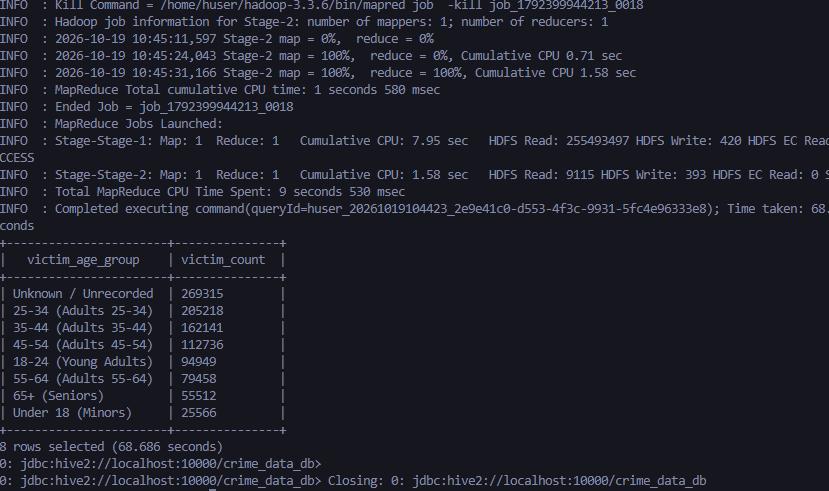
\includegraphics[max width=0.92\linewidth, max height=5.5cm, keepaspectratio]{images/ex1_09_victim_age_groups.png}
\end{center}
\textbf{Résultat :} Les jeunes adultes âgés de \textbf{25 à 34 ans} représentent la tranche la plus touchée (205,218 victimes, soit 20.42\%), suivis par les 35--44 ans (16.14\%). La catégorie inconnue (26.8\%) correspond aux crimes sans victime physique directe (vols de véhicules en stationnement, dégradations de biens commerciaux).

% ------------------------------------------------------------------------------
\section*{10. Surveillance de l'Exécution sur le Cluster YARN}
% ------------------------------------------------------------------------------
\textbf{Objectif :} Vérification de l'exécution distribuée des jobs MapReduce via l'interface Web du ResourceManager YARN (Port 8088).

\begin{center}
    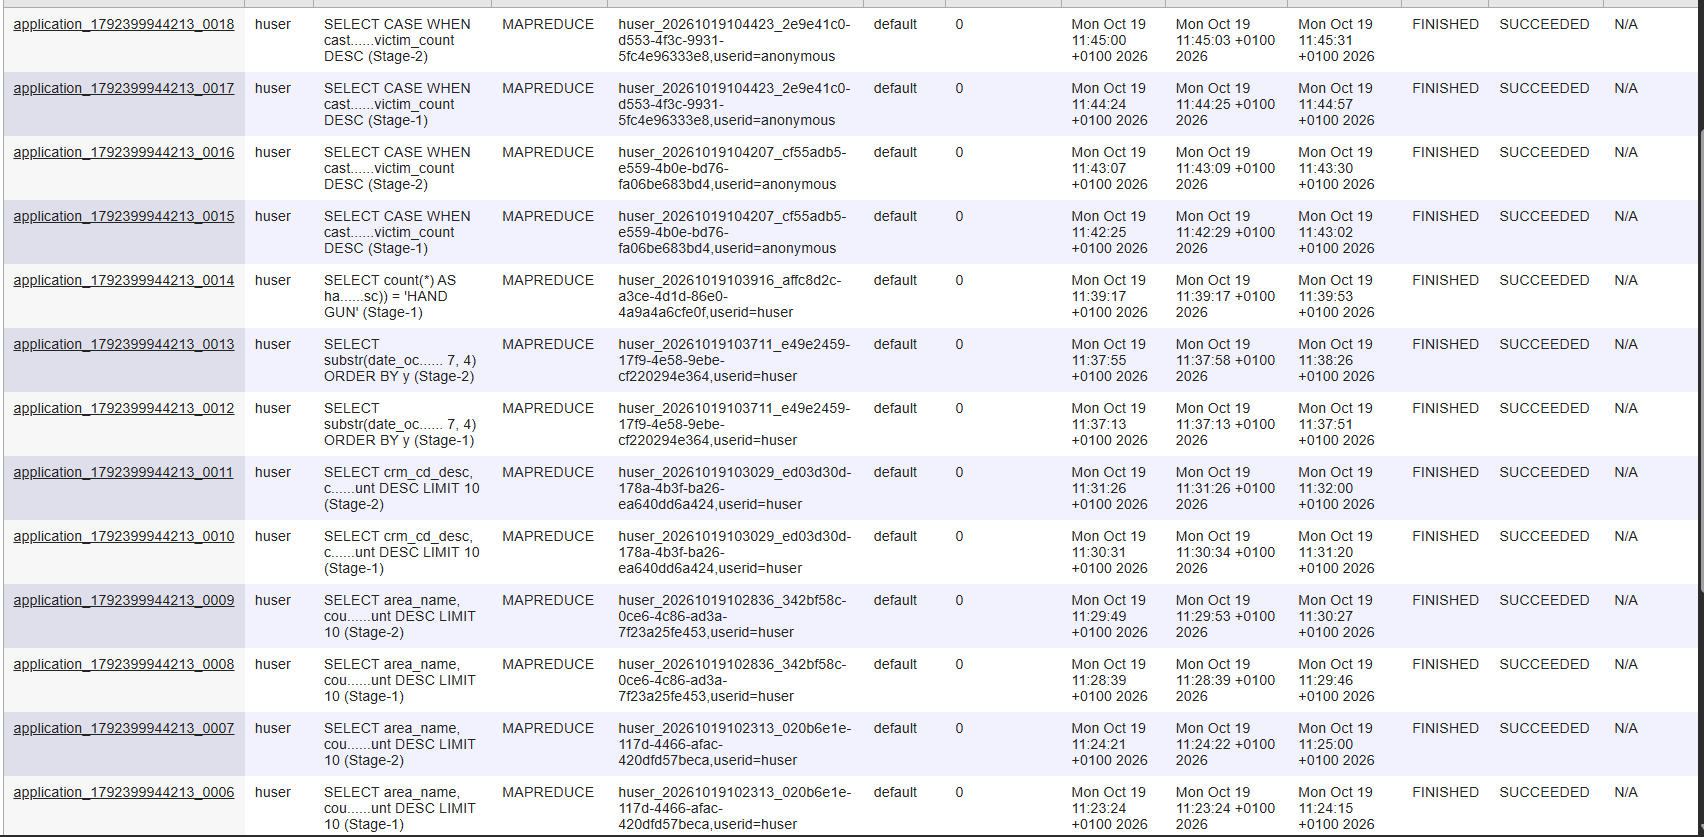
\includegraphics[max width=0.92\linewidth, max height=5.5cm, keepaspectratio]{images/ex1_10_yarn_job_execution.png}
\end{center}
\textbf{Résultat :} Toutes les requêtes ont été parallélisées et distribuées avec succès sur les nœuds workers (\texttt{worker1} et \texttt{worker2}) avec le statut \texttt{SUCCEEDED}.

\end{document}
